\documentclass[11pt]{article}
\usepackage[margin=2cm,a4paper]{geometry}
\usepackage{graphicx}
\usepackage{authblk}
\usepackage{url}
\usepackage{array}
\usepackage{amsfonts}
\usepackage{multirow}
\usepackage{amsmath}
\usepackage[usenames, dvipsnames]{color, colortbl}
\usepackage[normalem]{ulem}

\usepackage[outdir=./img/]{epstopdf}
\usepackage{epsfig}

\usepackage{tikz}
\usetikzlibrary{fit,positioning}
\usetikzlibrary{arrows}

\makeatletter
\def\title#1{\gdef\@title{Supplement to: ``#1''}}
\makeatother
\renewcommand{\thetable}{S\arabic{table}}%
\renewcommand{\thefigure}{S\arabic{figure}}%
\renewcommand{\thepage}{S\arabic{page}}

\setlength\parindent{0pt}


% supplement referencing
\usepackage{subcaption}
%\usepackage{cleveref}

% tablet style table
 \usepackage{booktabs}
 
\title{Triqler for Protein Summarization of Data from Data Independent Aquisition Mass Spectrometry}
\author{Patrick Truong \and Matthew The \and Lukas K\"{a}ll}


\begin{document}

\maketitle

\section*{Note S1: xxx}
\label{sec:fc-eval}


\iffalse
\subsection*{Fold change distributions}
\begin{figure}[hbt]
    \centering
    \begin{tabular}{lclc} 
        A & 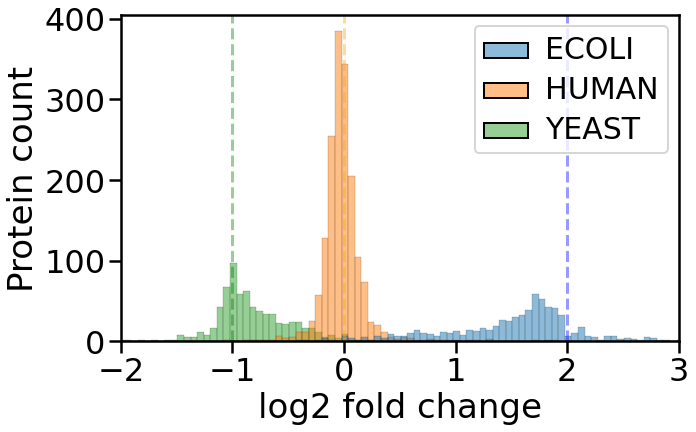
\includegraphics[width=0.4\linewidth]{../../result/report_plots/osw_triqler_intensity.png} & 
        E & 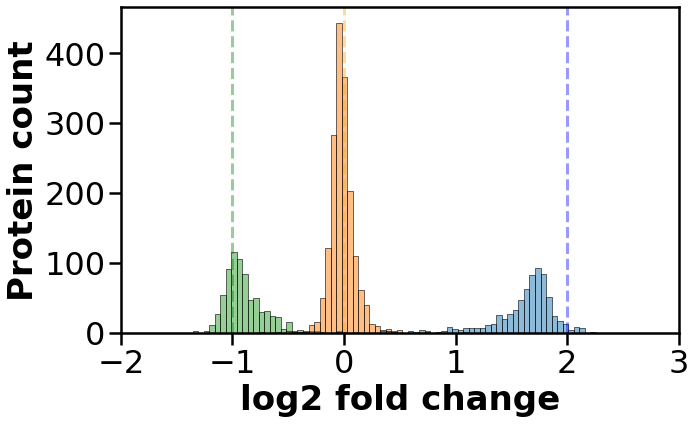
\includegraphics[width=0.4\linewidth]{../../result/report_plots/diann_triqler_intensity.png} \\ 
        B & 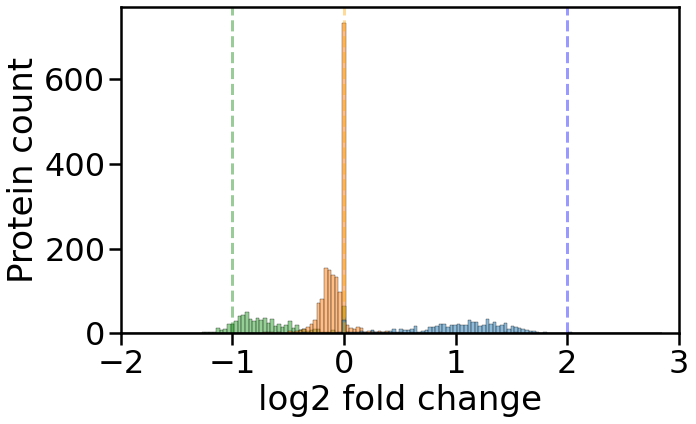
\includegraphics[width=0.4\linewidth]{../../result/report_plots/osw_msqrobsum_intensity.png} & 
        F & 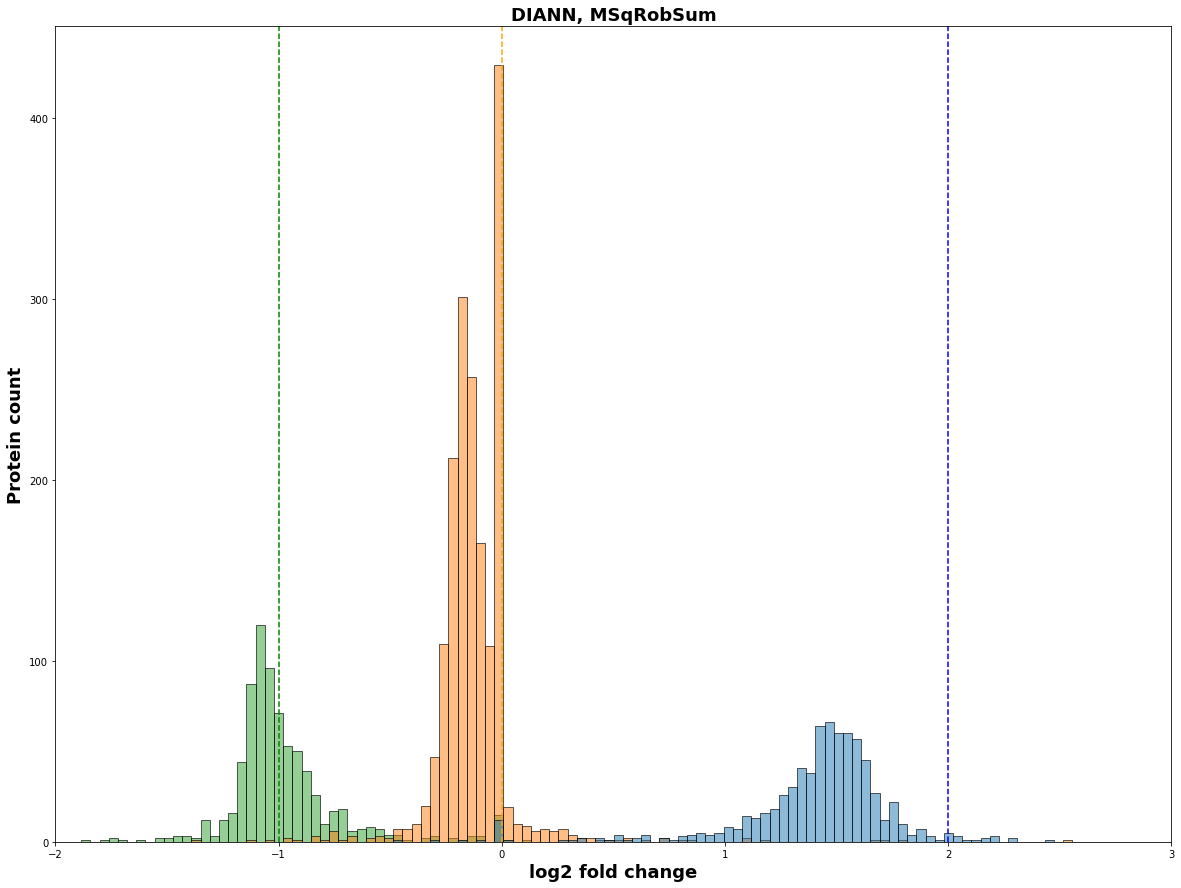
\includegraphics[width=0.4\linewidth]{../../result/report_plots/diann_msqrobsum_intensity.png} \\ 
        C & 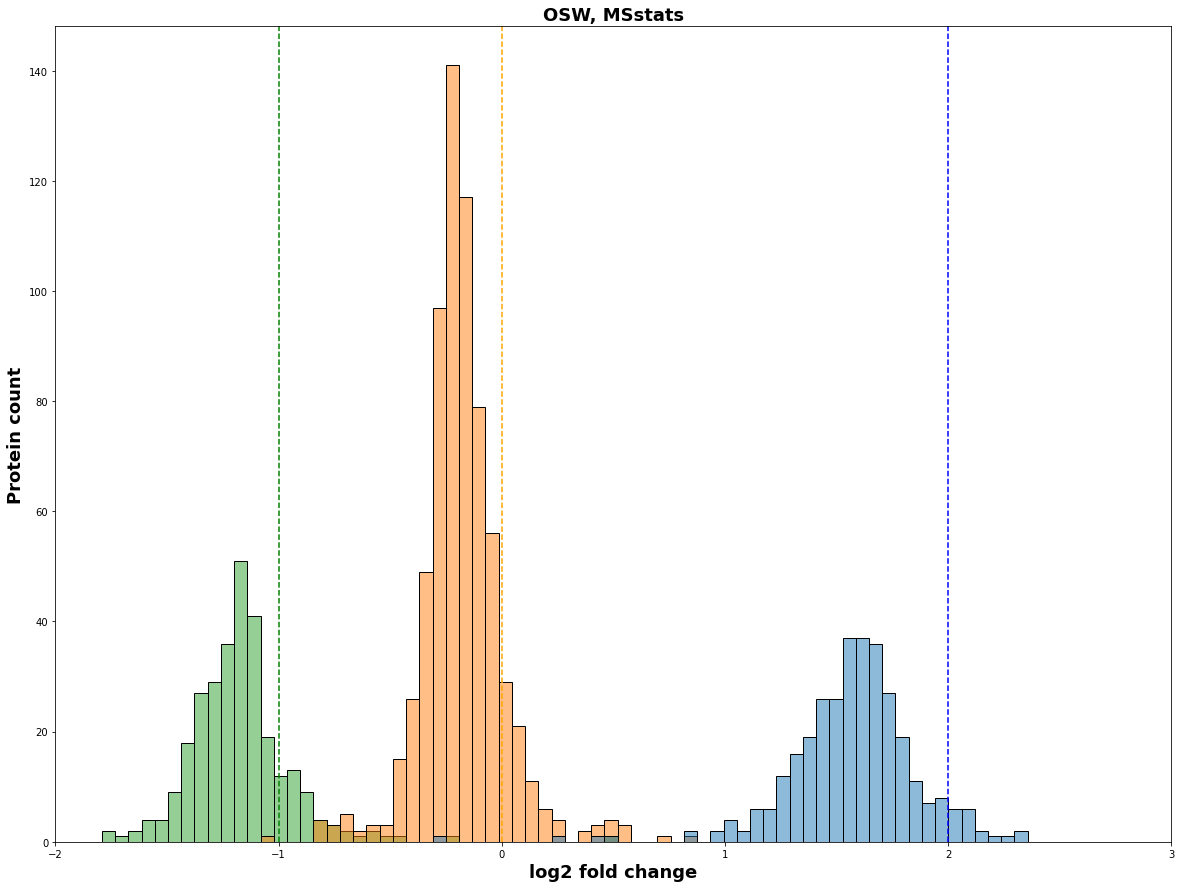
\includegraphics[width=0.4\linewidth]{../../result/report_plots/osw_msstats_intensity.png} & 
        G & 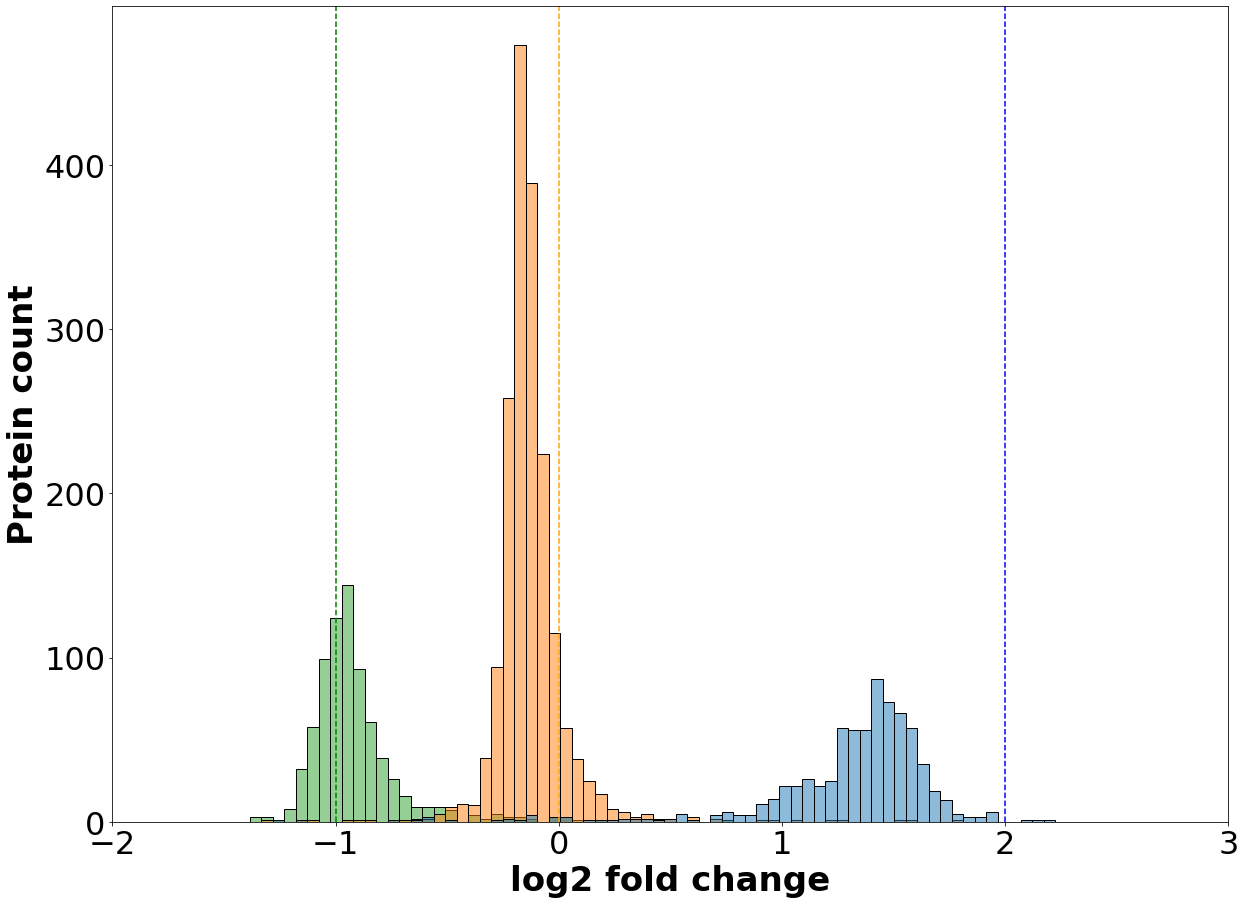
\includegraphics[width=0.4\linewidth]{../../result/report_plots/diann_msstats_intensity.png} \\ 
        D & 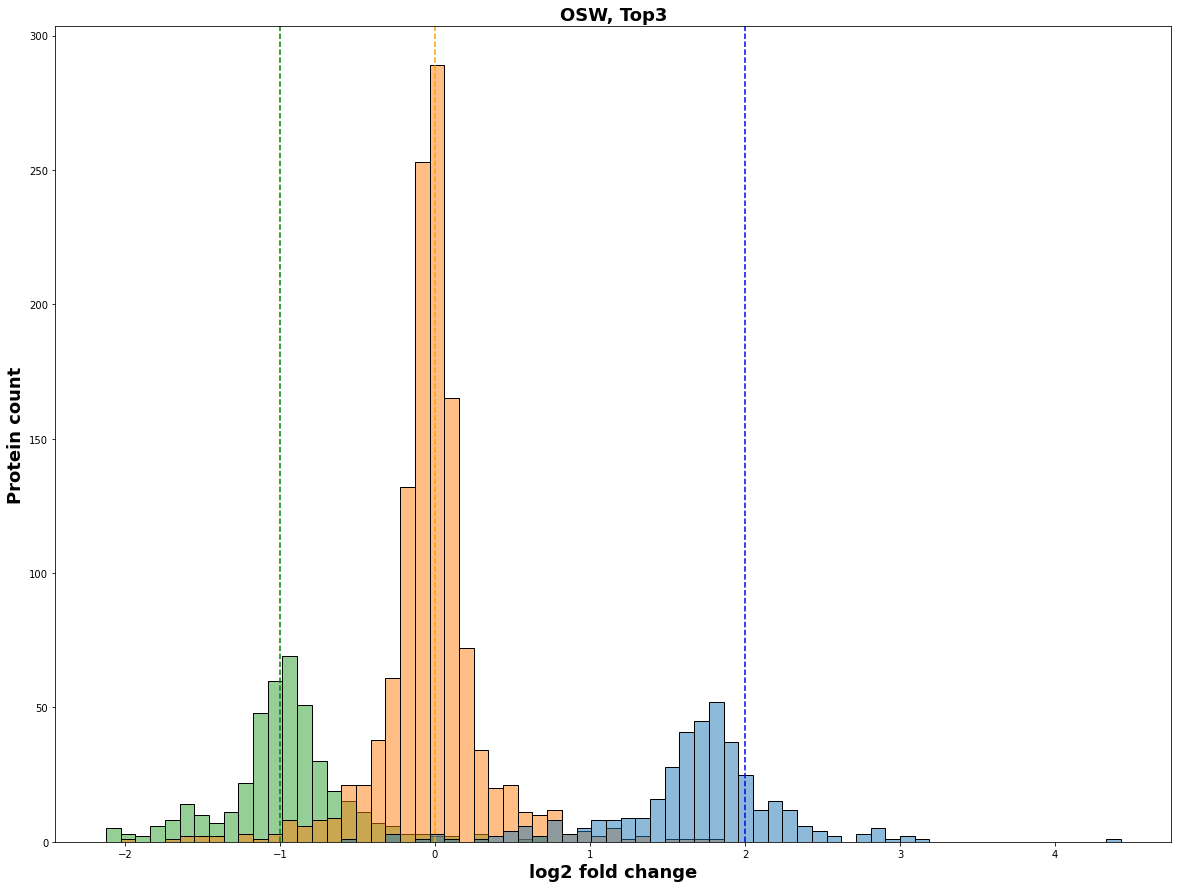
\includegraphics[width=0.4\linewidth]{../../result/report_plots/osw_top3_intensity.png} &
        H & 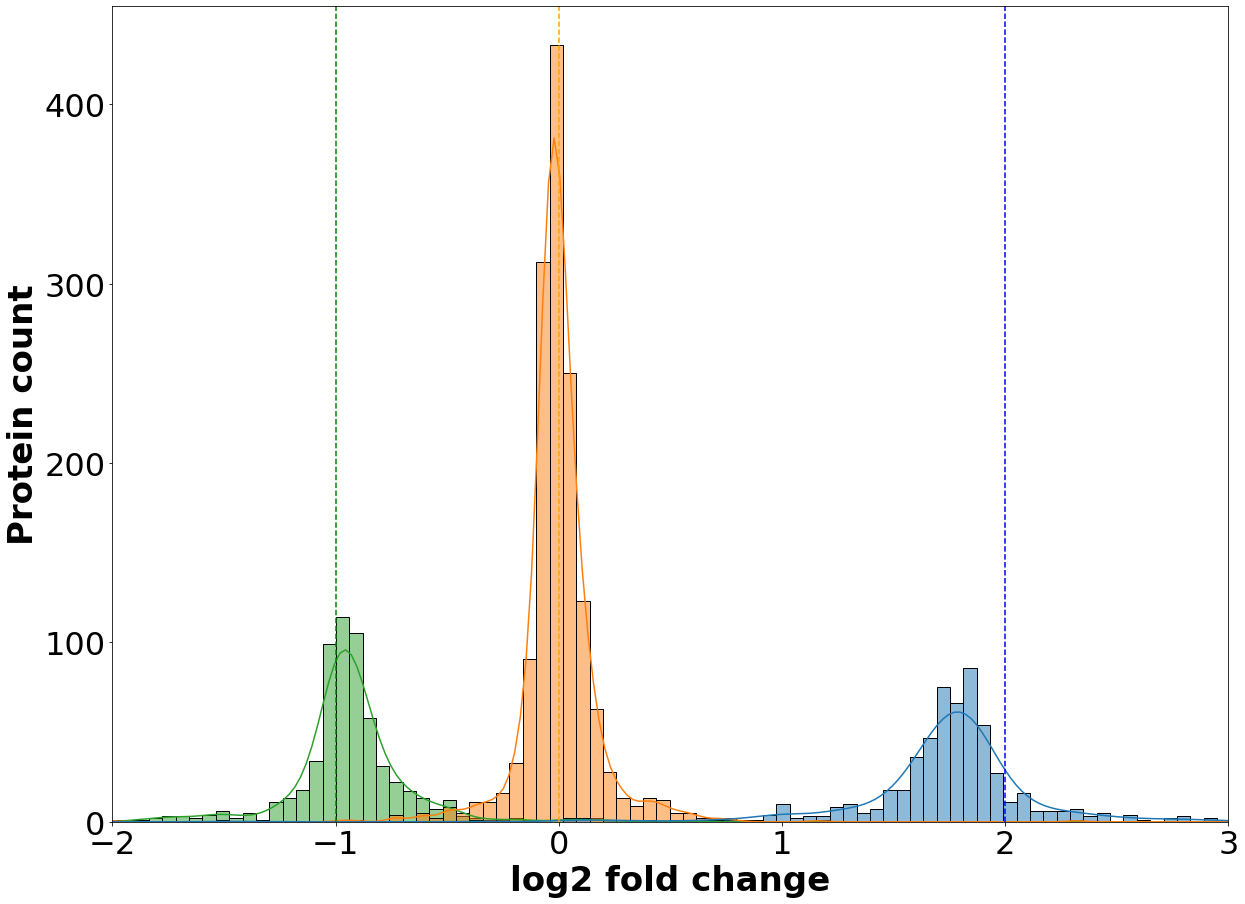
\includegraphics[width=0.4\linewidth]{../../result/report_plots/diann_top3_intensity.png} 
    \end{tabular}
   
    \caption{{\bf Comparison of reported fold change distributions.} We used peptide data from (A-D) DDA spectrum libraries and (E-H) psedo spectra as generated by 
    (A,E) Triqler, (B,F) MSqRobSum, (C,G) MSstats, and (D,H) Top-3. \label{fig:fc_histogram_again}}
\end{figure}

\fi


\iffalse
\subsubsection*{Differential abundance}
\begin{figure}[hbt]
    \centering
    \begin{tabular}{lclc} 
        A & 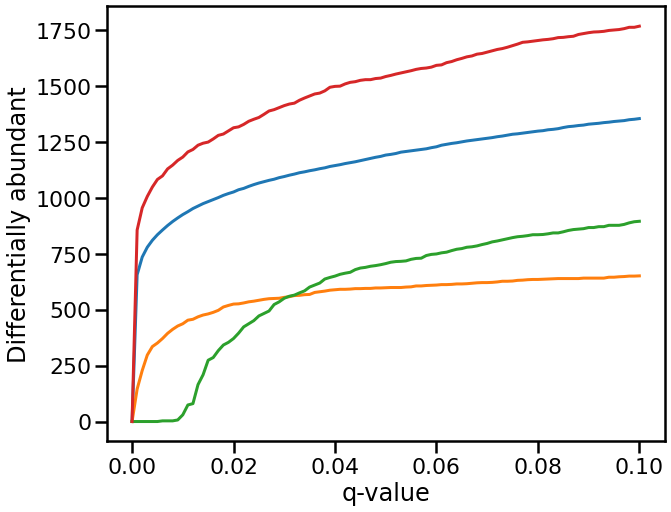
\includegraphics[width=0.4\linewidth]{../../result/report_plots/osw_de_all.png} & 
        E & 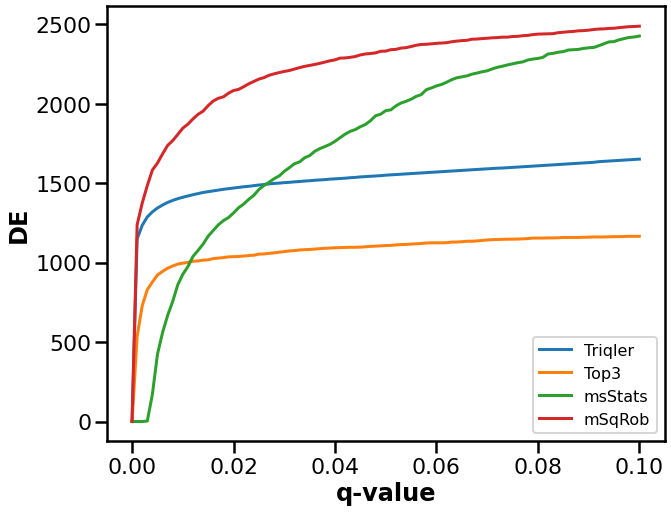
\includegraphics[width=0.4\linewidth]{../../result/report_plots/diann_de_all.png} \\ 
        B & 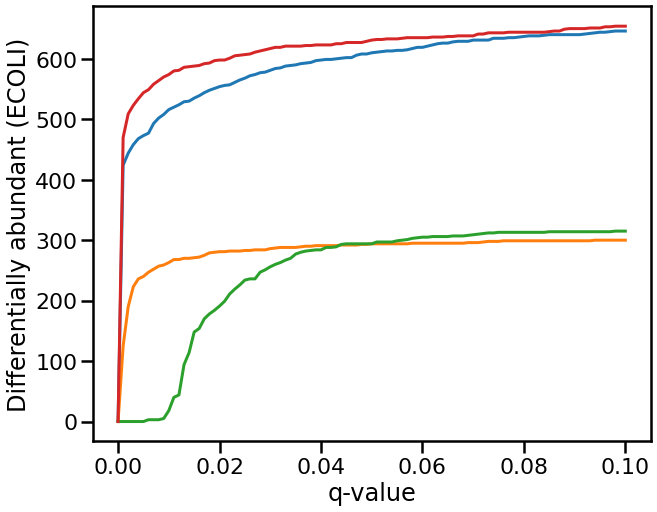
\includegraphics[width=0.4\linewidth]{../../result/report_plots/osw_de_ecoli.png} & 
        F & 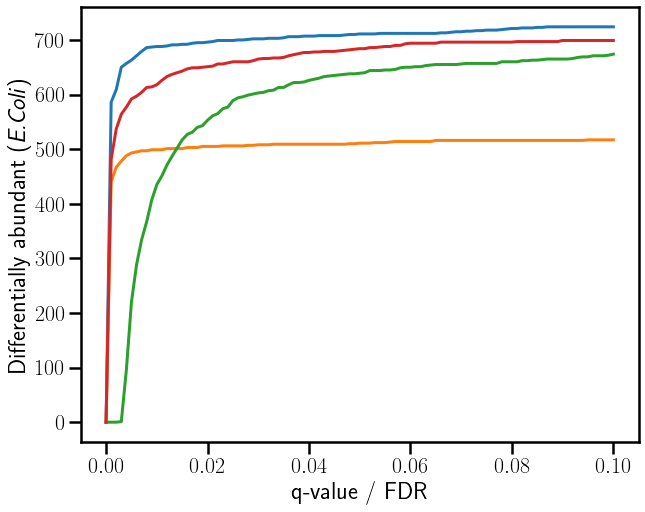
\includegraphics[width=0.4\linewidth]{../../result/report_plots/diann_de_ecoli.png} \\ 
        C & 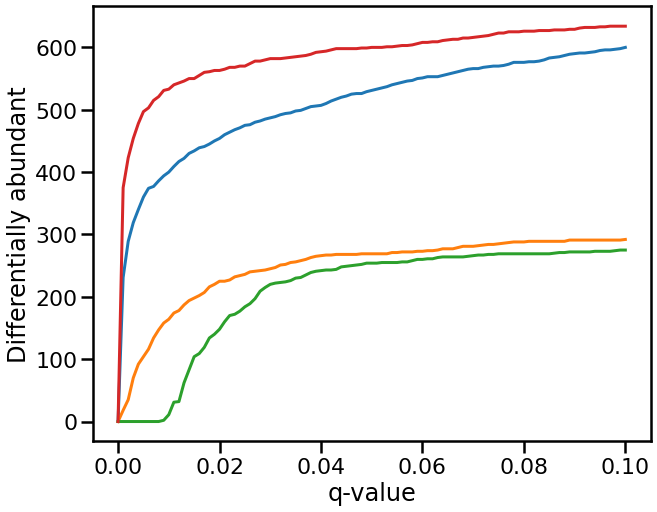
\includegraphics[width=0.4\linewidth]{../../result/report_plots/osw_de_yeast.png} & 
        G & 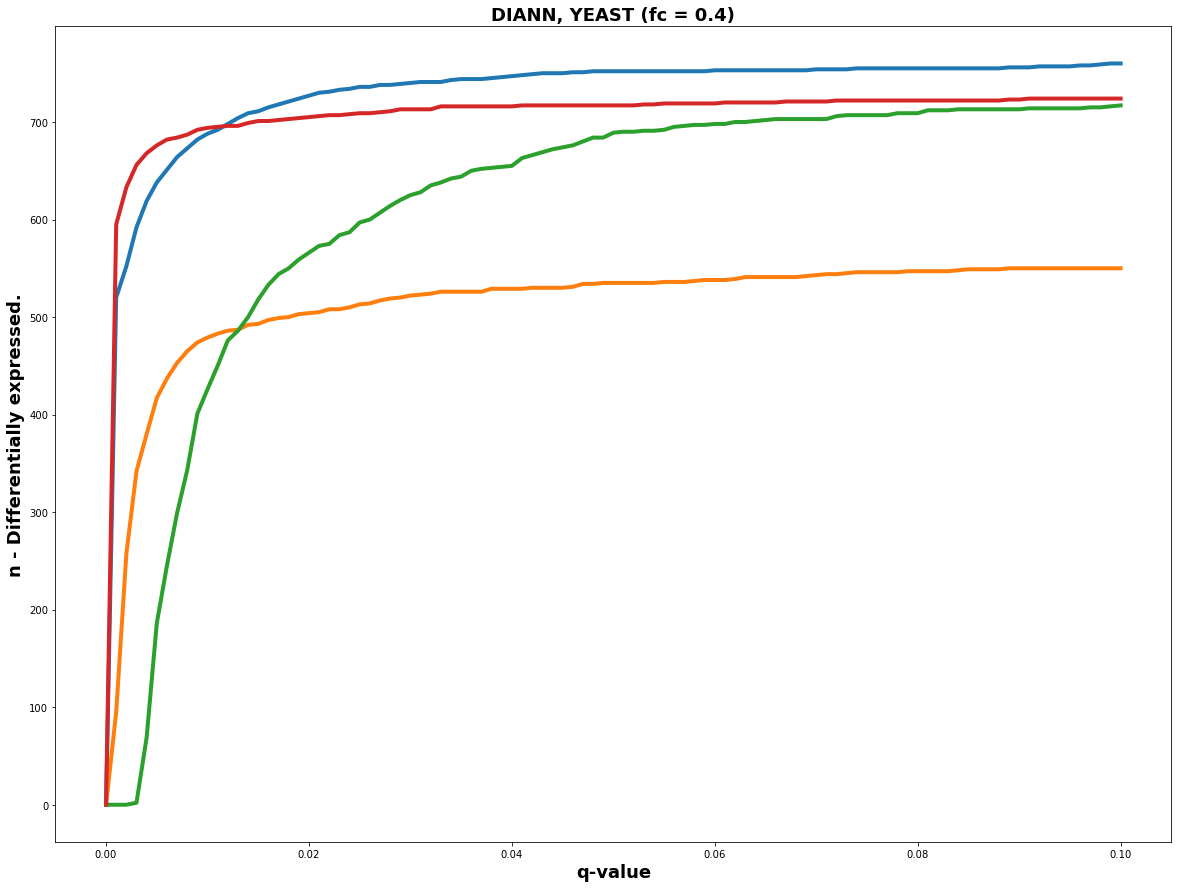
\includegraphics[width=0.4\linewidth]{../../result/report_plots/diann_de_yeast.png} \\ 
        D & 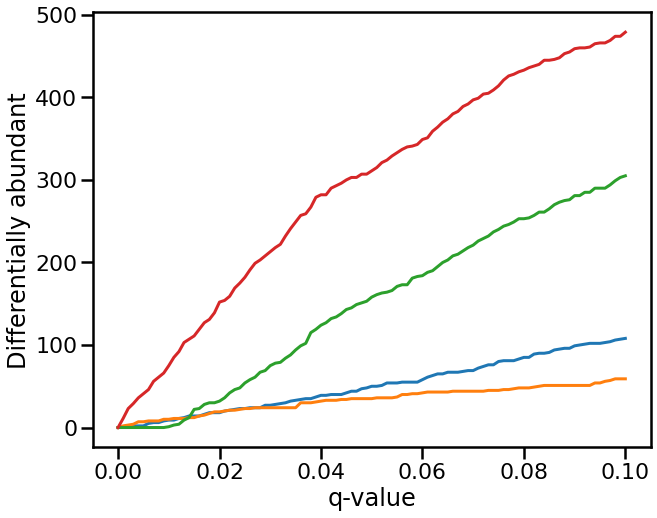
\includegraphics[width=0.4\linewidth]{../../result/report_plots/osw_de_human.png} &
        H & 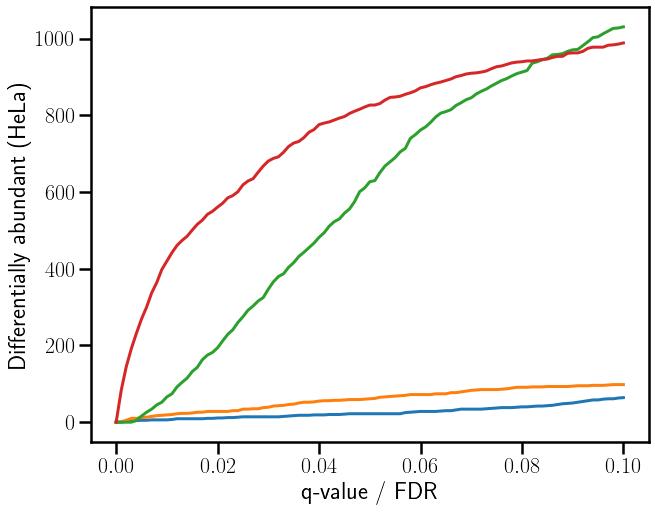
\includegraphics[width=0.4\linewidth]{../../result/report_plots/diann_de_human.png} 
    \end{tabular}
    \caption{{\bf Comparison of reported differential abundance.} Differential abundance is reported for (A-D) DDA spectrum libraries and (E-H) pseudo spectra for each proteome 
    (A,E) All, (B,F) ECOLI, (C,G) YEAST, and (D,H) HUMAN. \label{fig:da_lineplot_find_a_better_label}}
\end{figure}
\fi


\subsubsection*{Comparison of ability to differentiate differentially abundant proteins}
\begin{figure}[hbt]
    \centering
    \begin{tabular}{lclc} 
        A & 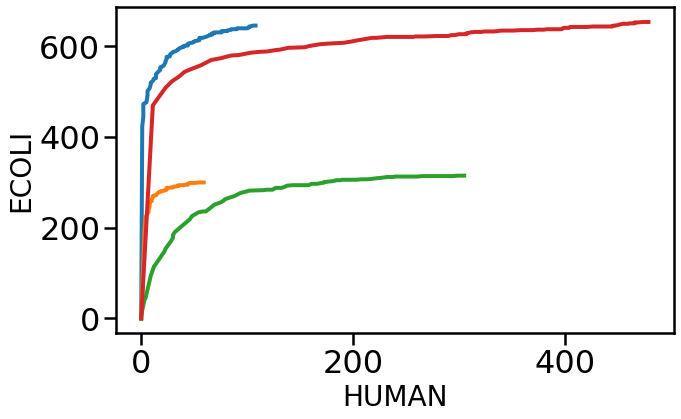
\includegraphics[width=0.4\linewidth]{../../result/report_plots/osw_de_human_vs_ecoli.png} & 
        D & 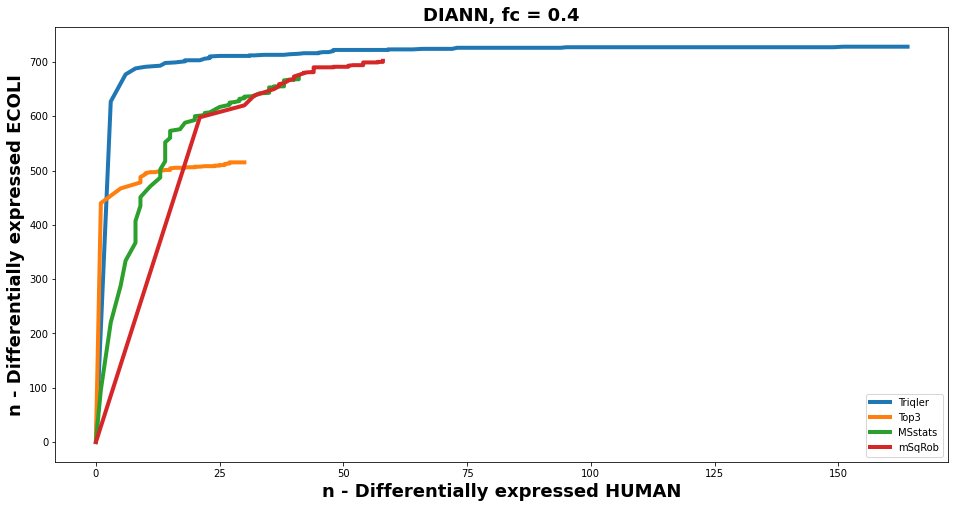
\includegraphics[width=0.4\linewidth]{../../result/report_plots/diann_de_human_vs_ecoli.png} \\ 
        B & 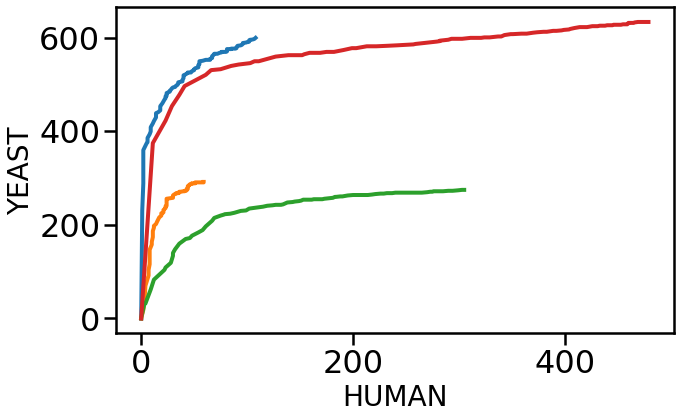
\includegraphics[width=0.4\linewidth]{../../result/report_plots/osw_de_human_vs_yeast.png} & 
        E & 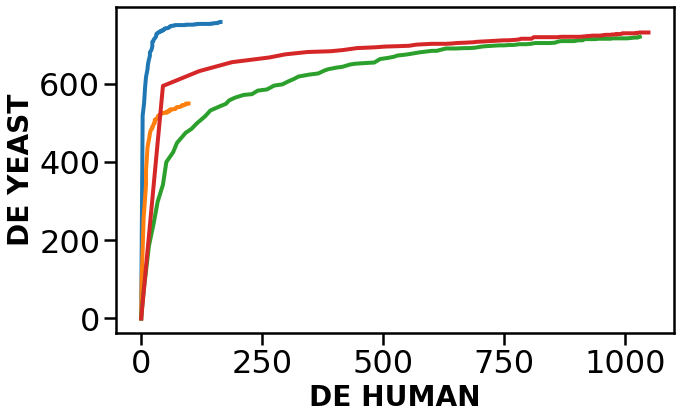
\includegraphics[width=0.4\linewidth]{../../result/report_plots/diann_de_human_vs_yeast.png} \\
        C & 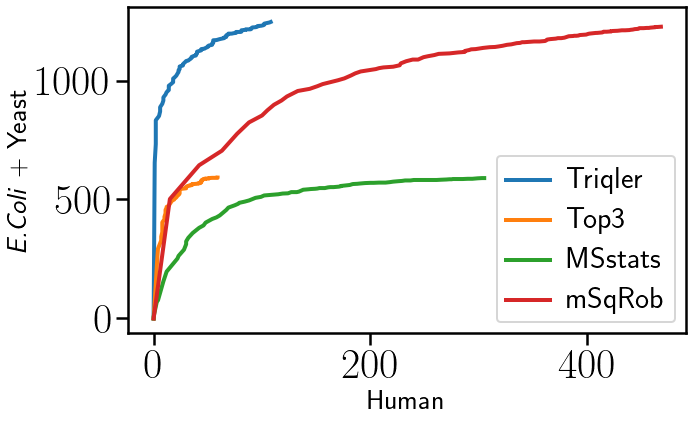
\includegraphics[width=0.45\linewidth]{../../result/report_plots/osw_de_human_vs_ecoli_and_yeast.png} & 
        F & 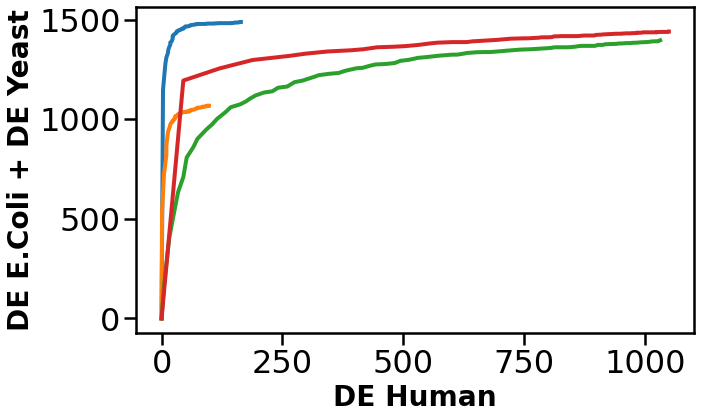
\includegraphics[width=0.45\linewidth]{../../result/report_plots/diann_de_human_vs_ecoli_and_yeast.png} \\ 

    \end{tabular}
    \caption{{\bf Comparison of ability to differentiate differentially abundant proteins} We plotted the number of reported differentially abundant  {\em E. Coli} and Yeast proteins as a function of number of proteins from the HeLa background when sorting according to significance for (A) DDA generated spectral libraries and (B) DIA-Umpire geneated Pseudo spectra. For the test we selected a fold-change treshold of 0.4 for Triqler. \label{fig:diff_vs_hela_find_a_better_label}}
\end{figure}

\iffalse

\subsubsection*{Comparison of statistical calibration}
\begin{figure}[hbt]
    \centering
    \centering
    \begin{tabular}{lclc} 
        %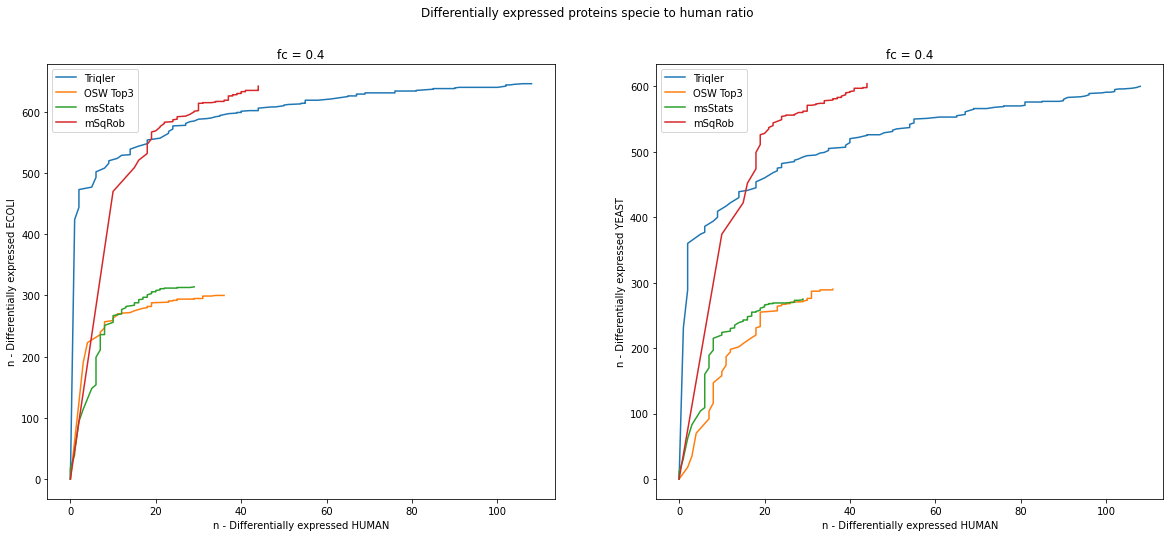
\includegraphics[width=0.3\linewidth]{../../result/report_plots/de_human_vs_de_specie.png} & 
        %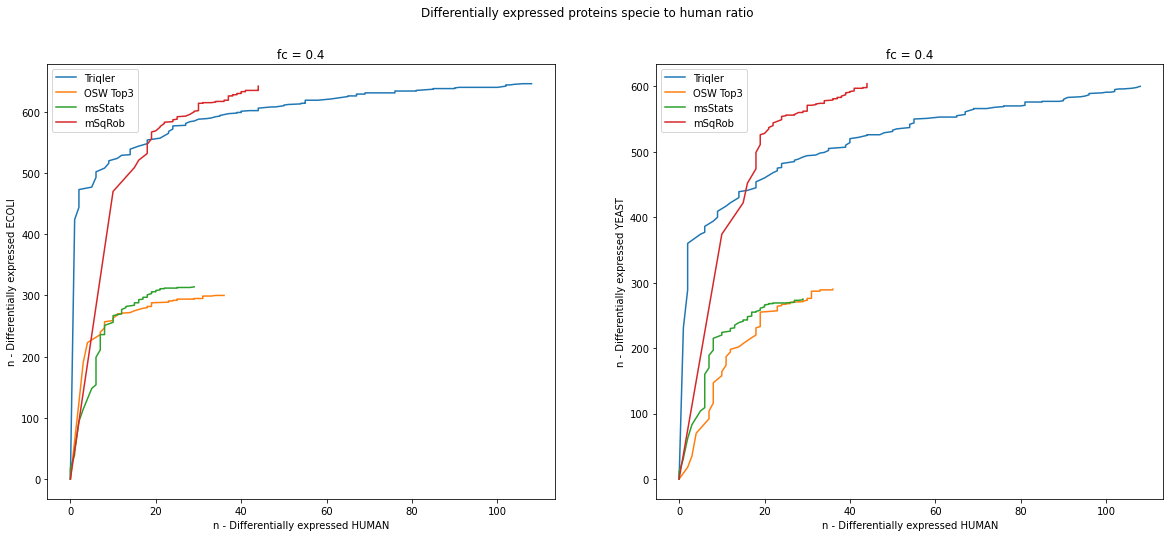
\includegraphics[width=0.3\linewidth]{../../result/report_plots/de_human_vs_de_specie.png} \\ 
        %A & B
        % A 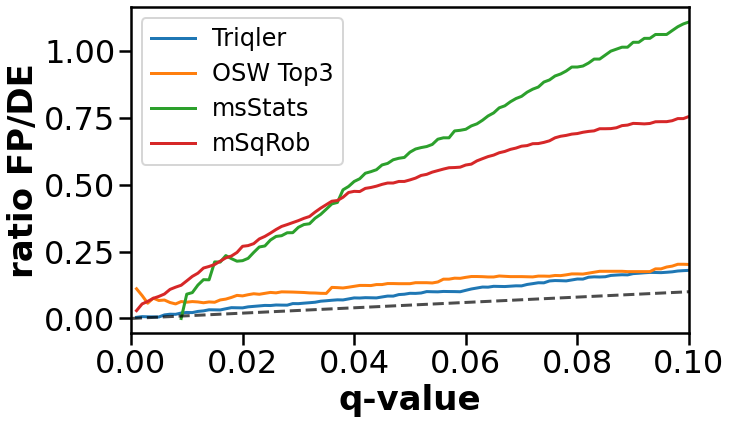
\includegraphics[width=0.5\linewidth]{../../result/report_plots/osw_FP_DE_yeast.png} & &%\includegraphics[width=0.3\linewidth]{} & 
        % D 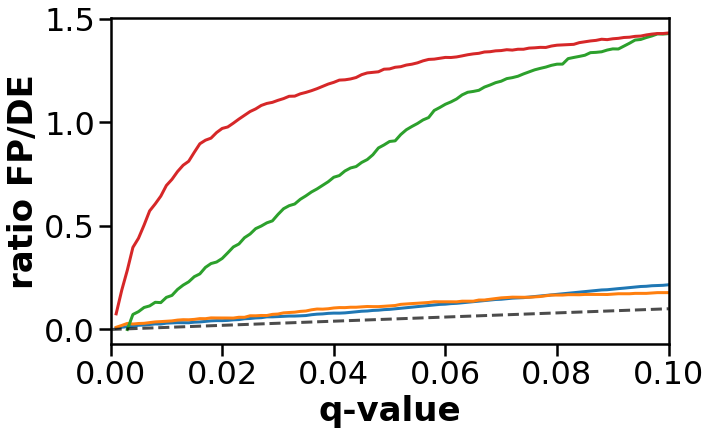
\includegraphics[width=0.5\linewidth]{../../result/report_plots/diann_FP_DE_yeast.png} & \\%\includegraphics[width=0.3\linewidth]{} \\ 
        % B 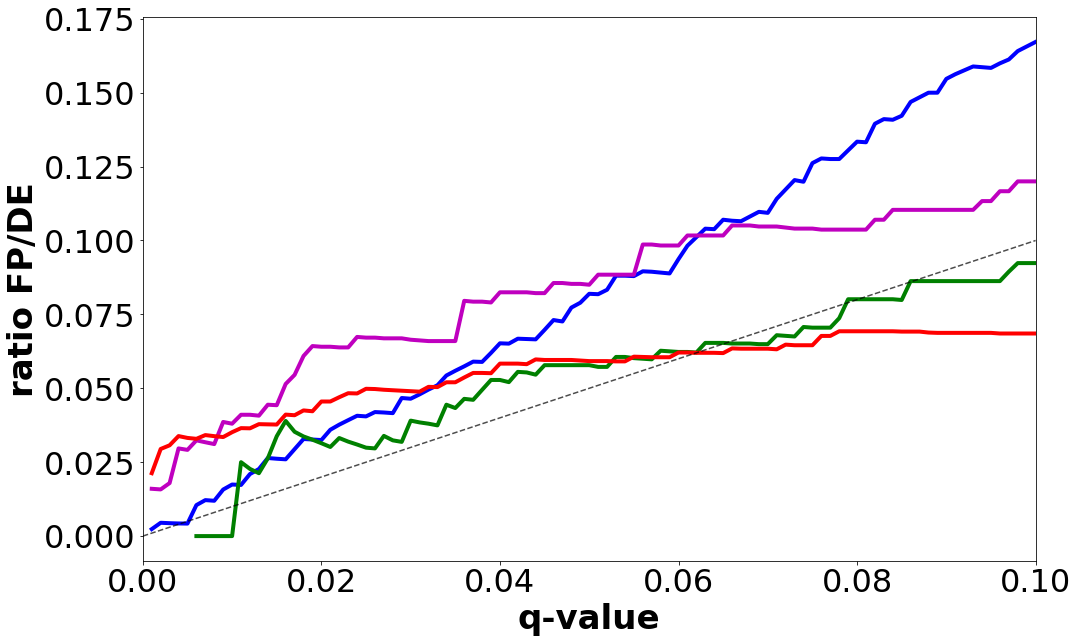
\includegraphics[width=0.5\linewidth]{../../result/report_plots/osw_FP_DE_ecoli.png} & &%\includegraphics[width=0.3\linewidth]{} & 
        % E 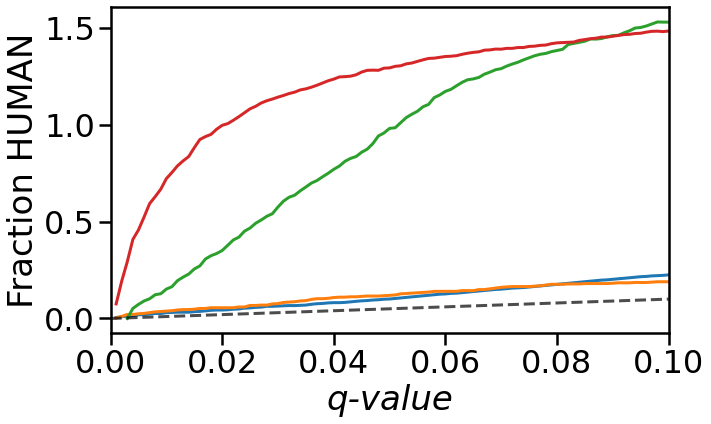
\includegraphics[width=0.5\linewidth]{../../result/report_plots/diann_FP_DE_ecoli.png} & \\%\includegraphics[width=0.3\linewidth]{} \\ 
        A 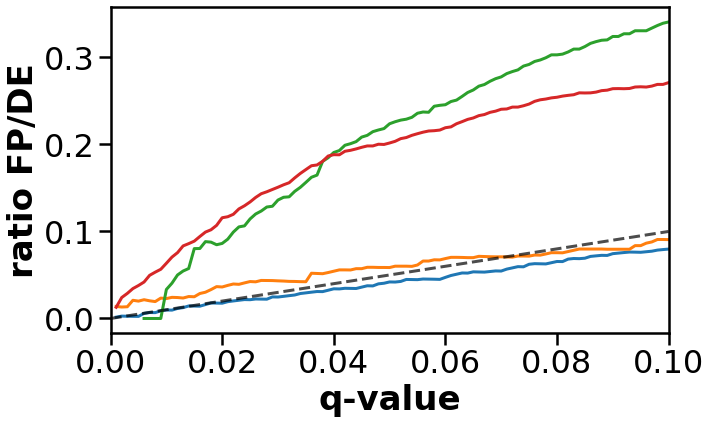
\includegraphics[width=0.5\linewidth]{../../result/report_plots/osw_FP_DE_all.png} & &%\includegraphics[width=0.3\linewidth]{} & 
        B 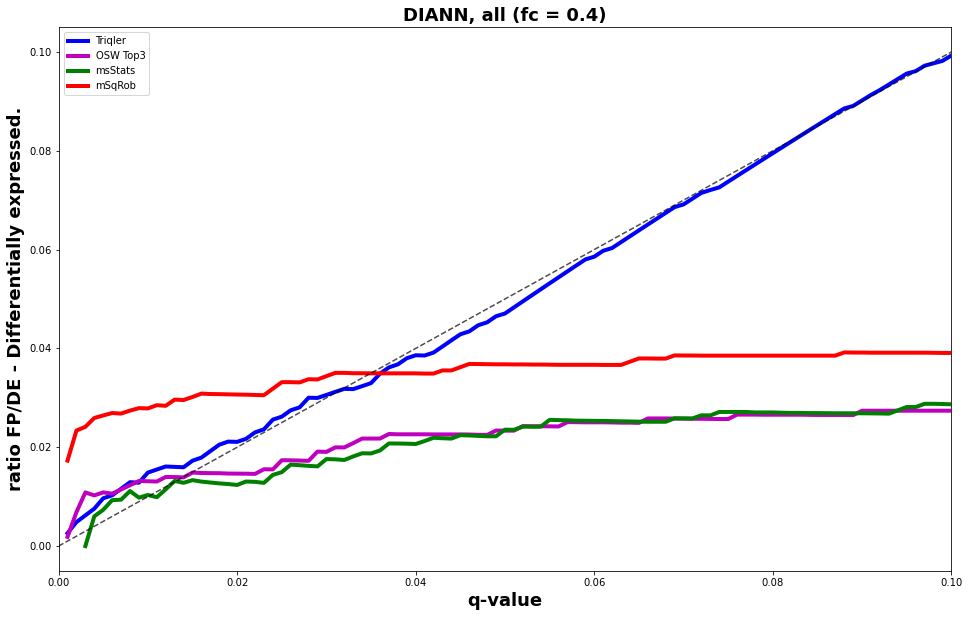
\includegraphics[width=0.5\linewidth]{../../result/report_plots/diann_FP_DE_all.png} & \\%\includegraphics[width=0.3\linewidth]{} \\ 
    \end{tabular}
  \caption{{\bf Comparison of calibration of the compared summarization methods.} We plotted the fraction of reported differentially abundant HeLa proteins as a function of $q$~value for (A) DDA generated spectral libraries and (B) DIA-Umpire geneated Pseudo spectra. \label{fig:frac_hela_vs_fdr_find_a_better_label}}
\end{figure}
\fi


\subsubsection*{Constant variance}
\begin{figure}[hbt]
    \centering
    \centering
    \begin{tabular}{lclc} 
        A 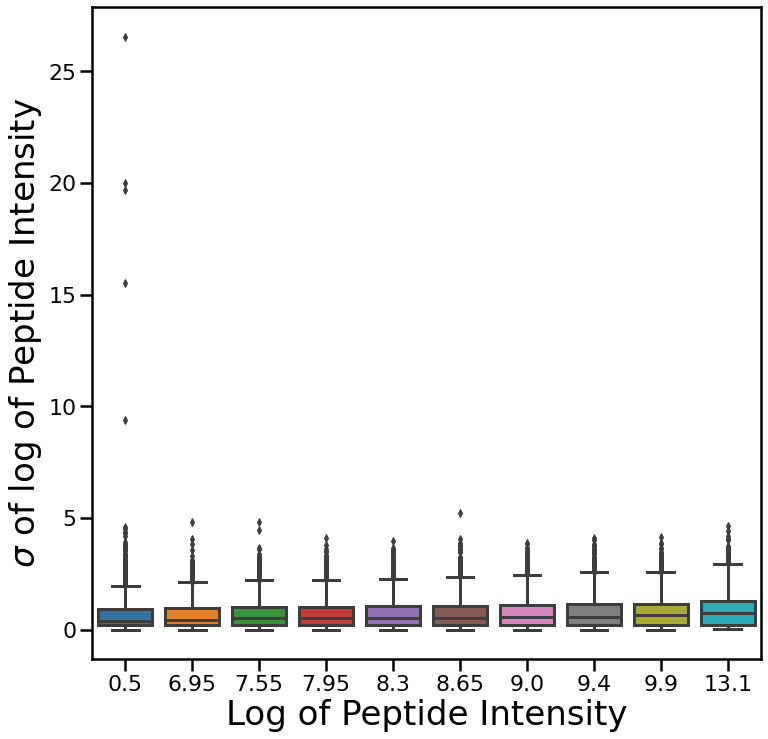
\includegraphics[width=0.5\linewidth]{../../result/mu_sigma_variance_plots/osw_log/osw_boxplot_qvalFiltered_pepFiltered_qbinned.png} & &%\includegraphics[width=0.3\linewidth]{} & 
        B 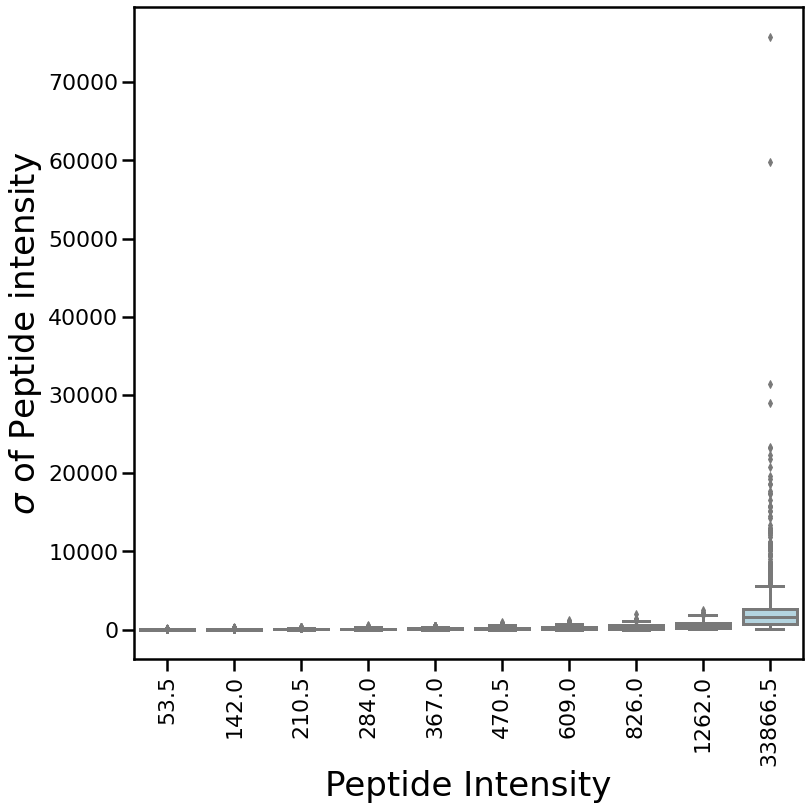
\includegraphics[width=0.5\linewidth]{../../result/mu_sigma_variance_plots/osw/osw_boxplot_nolog_qvalFiltered_pepFiltered_qbinned.png} & \\%\includegraphics[width=0.3\linewidth]{} \\ 
        C 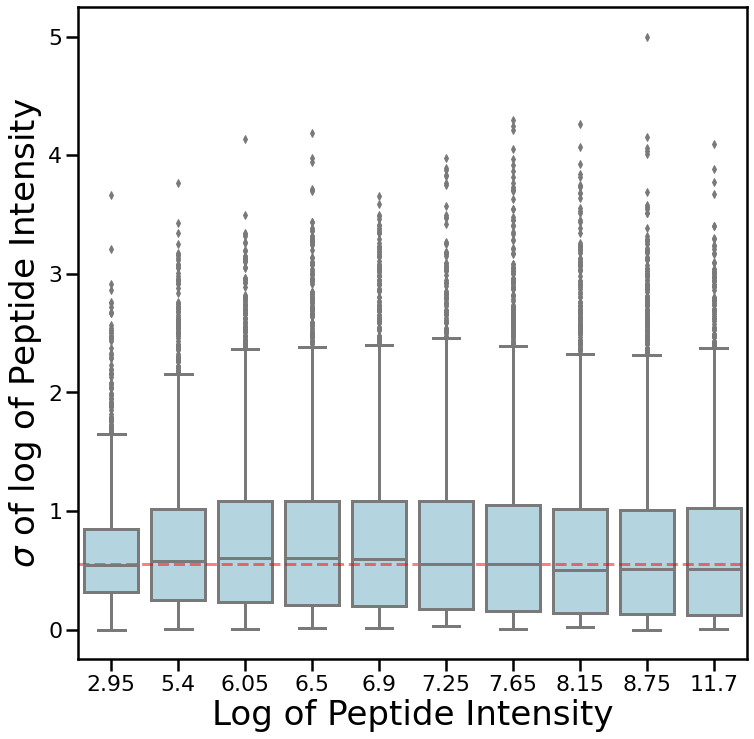
\includegraphics[width=0.5\linewidth]{../../result/mu_sigma_variance_plots/diann_log/diann_boxplot_qvalFiltered_pepFiltered_qbinned.png} & &%\includegraphics[width=0.3\linewidth]{} & 
        D 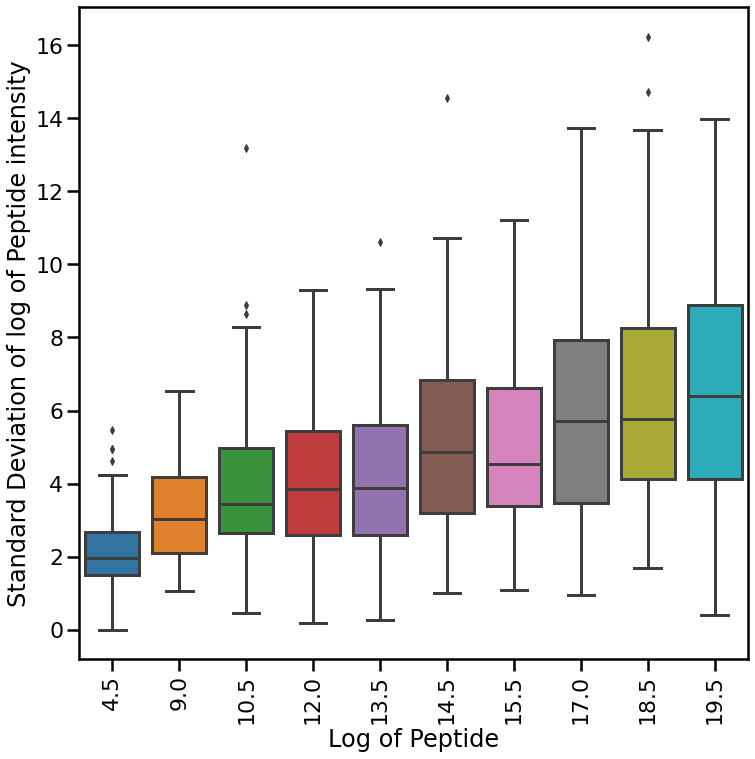
\includegraphics[width=0.5\linewidth]{../../result/mu_sigma_variance_plots/diann/diann_boxplot_nolog_qvalFiltered_pepFiltered_qbinned.png} & \\%\includegraphics[width=0.3\linewidth]{} \\ 
    \end{tabular}
  \caption{{\bf Uniform offset in standard deviation.} We plotted the standard deviation as a function of the mean of every peptide intensity in the TripleTOF6600 section of the LFQ Bench set  in a linear and log-log scale for (A-B) spectral library matching and (C-D) pseudo-spectra workflows.  We observe a nearly uniform offset in standard deviation across the intensity scale, demonstrating that $\log(\sigma) \approx \log(\mu) + \log(k)$ and hence   $\sigma \approx \mu k$. Linear scale plots are reported as reference.  \label{fig:mu_sigma_boxplot_find_a_better_label}}
\end{figure}


\iffalse
\begin{figure}[hbt]
    \centering
    \centering
    \begin{tabular}{lclc} 
        A 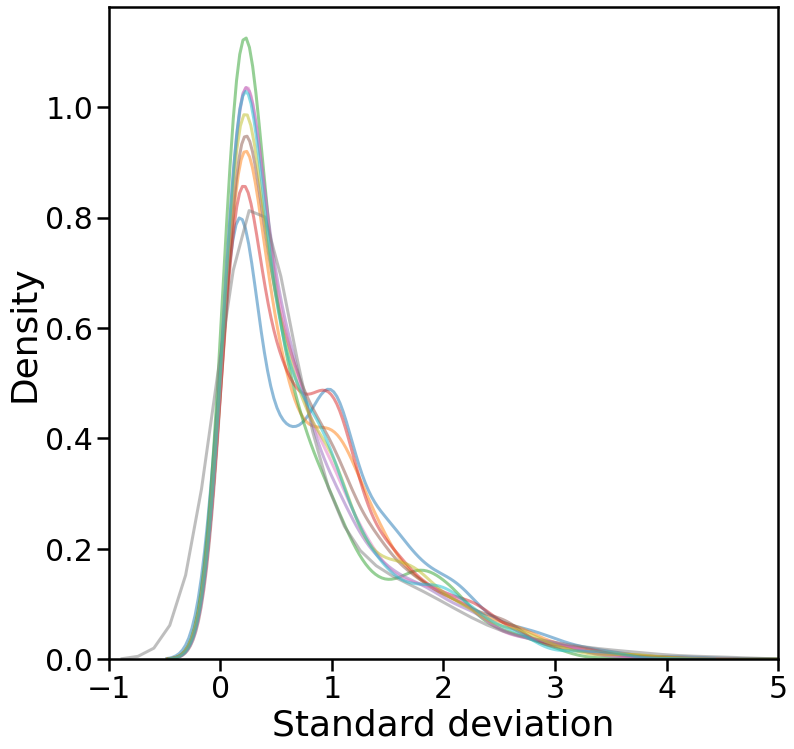
\includegraphics[width=0.5\linewidth]{../../result/mu_sigma_variance_plots/osw_log/osw_kde_qvalFiltered_pepFiltered_qbinned.png} & &%\includegraphics[width=0.3\linewidth]{} & 
        B 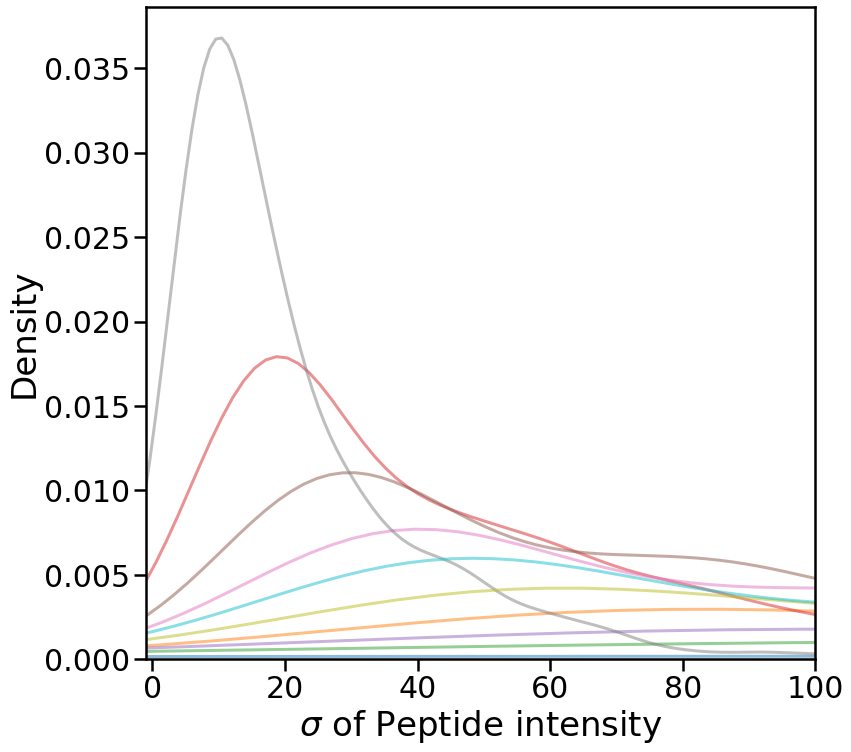
\includegraphics[width=0.5\linewidth]{../../result/mu_sigma_variance_plots/osw/osw_kde_nolog_qvalFiltered_pepFiltered_qbinned.png} & \\%\includegraphics[width=0.3\linewidth]{} \\ 
        C 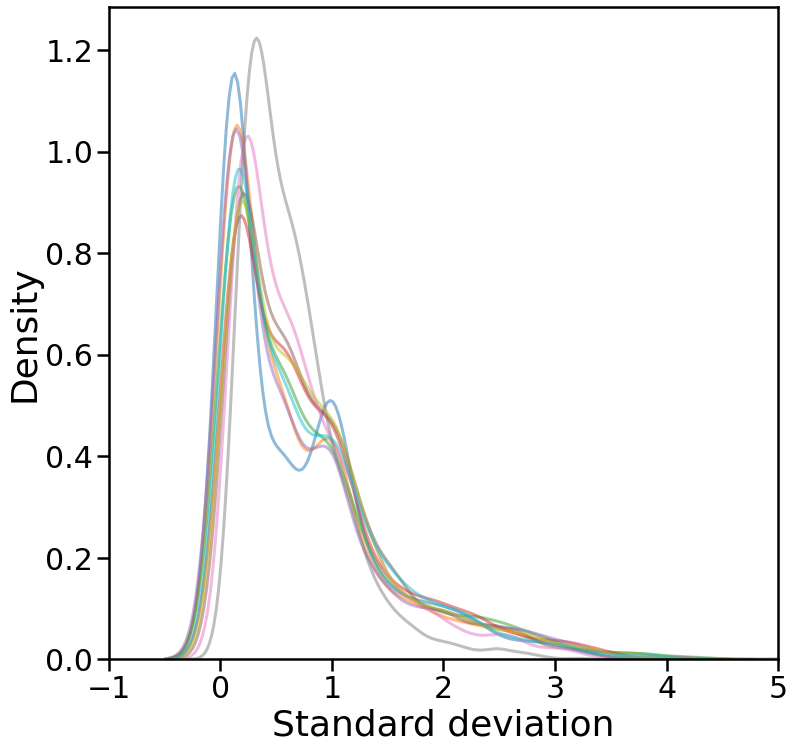
\includegraphics[width=0.5\linewidth]{../../result/mu_sigma_variance_plots/diann_log/diann_kde_qvalFiltered_pepFiltered_qbinned.png} & &%\includegraphics[width=0.3\linewidth]{} & 
    \end{tabular}
  \caption{{\bf Gaussian kernel density estimates of quantile binned peptide intensities.} We plotted the Gaussian kernel estimates of the quantile binned peptide intensities for (A-C) spectral library matching and (C-D) pseudo-spectra workflows. Approximately equal densities in the bins demonstrates the uniform offset in standard deviation across the intensity scale. \label{fig:mu_sigma_KDE_find_a_better_label}}
\end{figure}
\fi


% Please add the following required packages to your document preamble:


\begin{table}[hbt]
\centering
\begin{tabular}{llll}
\hline
        & Unfiltered & no\_shared & no\_shared\_IL\_equivalence \\ \hline
All     & 31 055     & 30 456     & 30 452                      \\
E. Coli & 4 391      & 4 306      & 4 306                       \\
Human   & 20 614     & 20 302     & 20 299                      \\
Yeast   & 6 050      & 5 848      & 5 847                       \\ \hline
\end{tabular}

  \caption{{\bf Protein count in the Uniprot FASTA protein database.} The database is a FASTA file with one protein sequence per gene for each species (UP000005640, UP000000625 and UP000002311. Acquired on 2021-06-16). The "no\_shared" filter is applied by splitting the protein sequences at amino acids "K" and "R" and keeping all the sequences with length $>$ 7 for each protein. We then mapped each sequence to all possible protein matchings and counted the how many proteins each split sequence was mapped to, and filtered so that each sequence only kept one protein match. Therefore, creating a database library with only one peptide sequence per protein. For the "no\_shared\_IL\_equivalence" all I are replaced by L before performing the filtering.    \label{table:uniprot_protein_count_find_a_better_label}}

\end{table}



\subsubsection*{Comparison of statistical calibration}
\begin{figure}[hbt]
    \centering
    \centering
    \begin{tabular}{lclc} 
        A 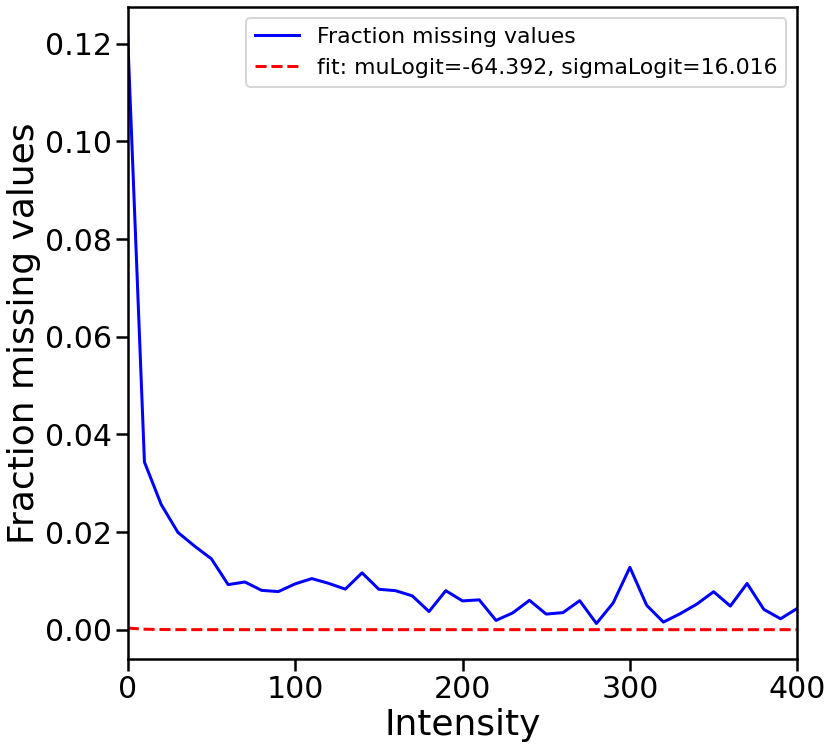
\includegraphics[width=0.5\linewidth]{../../result/report_plots/osw_fraction_missing_values.png} & &%\includegraphics[width=0.3\linewidth]{} & 
        B 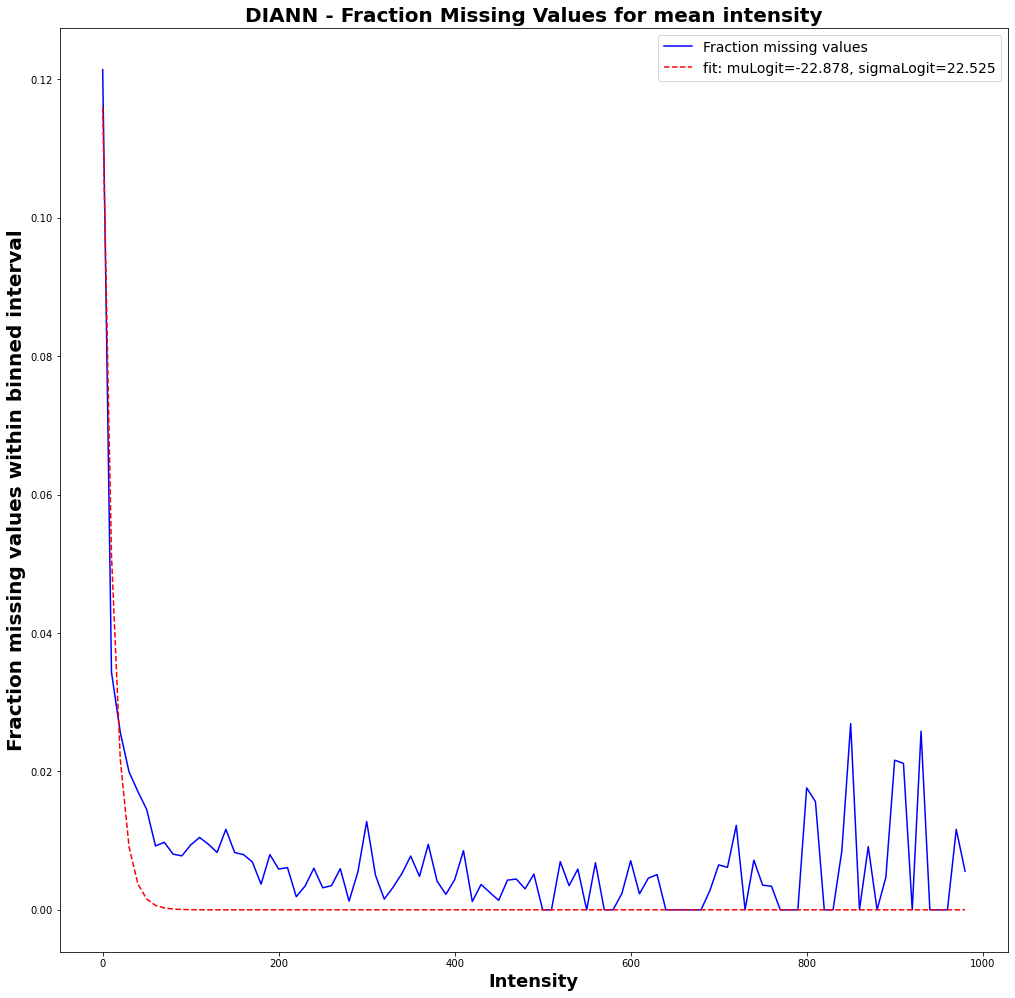
\includegraphics[width=0.5\linewidth]{../../result/report_plots/diann_fraction_missing_values.png} & \\%\includegraphics[width=0.3\linewidth]{} \\ 
    \end{tabular}
  \caption{{\bf Comparison of actual missing values against fit to the censored normal distribution used in triqler \cite{kall2020integrating}.} We imputed the missing values as the mean of sample peptide intensities and used these imputed values to approximate the missingness for a given intensity. We binned the intensities to an arbitrary small range and plotted the fraction os missing values for each intensity range. A cubic spline fit was used to fit the values against the mentioned censored normal distribution for (A) Spectral library matching  and (B) Pseudo spectra workflow. \label{fig:fraction_missing_values}}
\end{figure}



%\begin{figure}[hbt]
%    \centering
%    \centering
%    \begin{tabular}{lclc} 
%        A 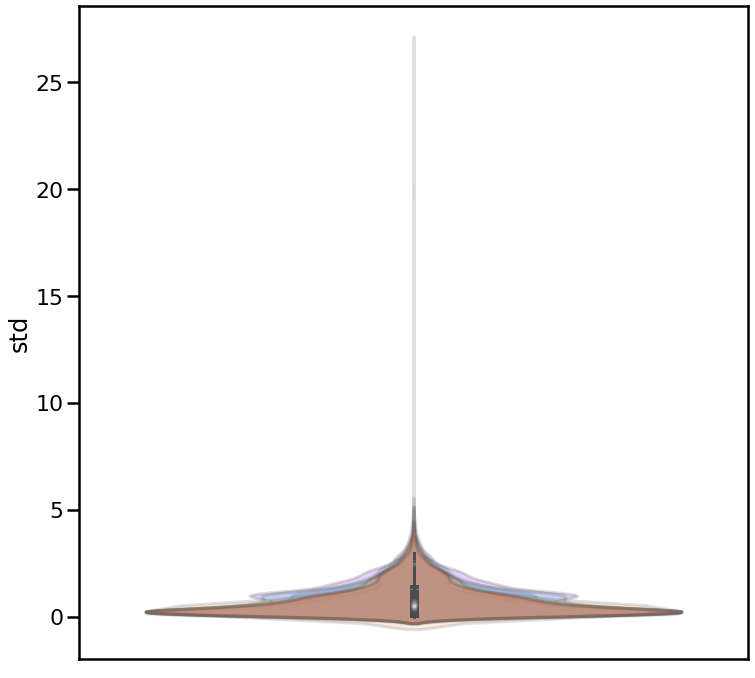
\includegraphics[width=0.5\linewidth]{../../result/mu_sigma_variance_plots/osw_log/osw_violinOverlap_qvalFiltered_pepFiltered_qbinned.png} & &%\includegraphics[width=0.3\linewidth]{} & 
%        B 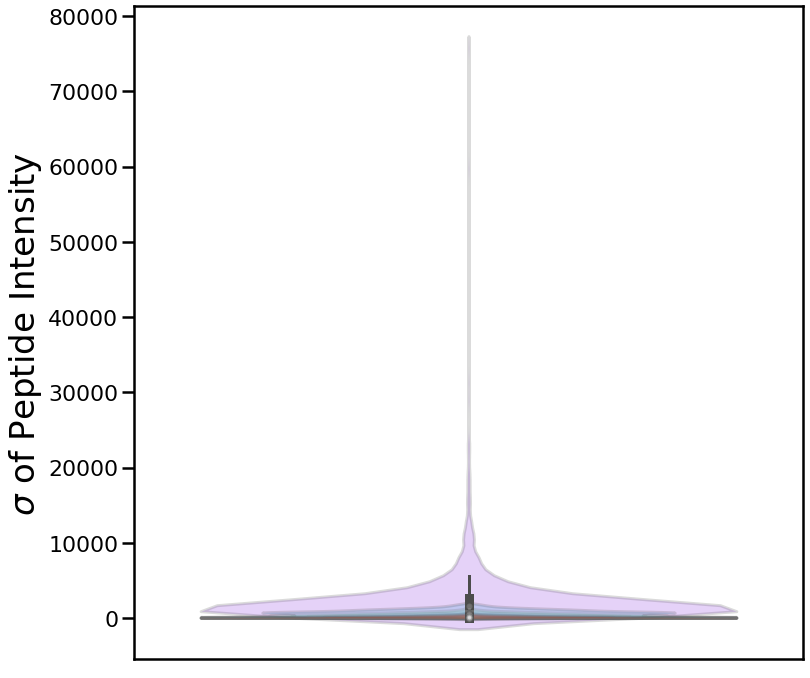
\includegraphics[width=0.5\linewidth]{../../result/mu_sigma_variance_plots/osw/osw_violinOverlap_nolog_qvalFiltered_pepFiltered_qbinned.png} & \\%\includegraphics[width=0.3\linewidth]{} \\ 
%        C 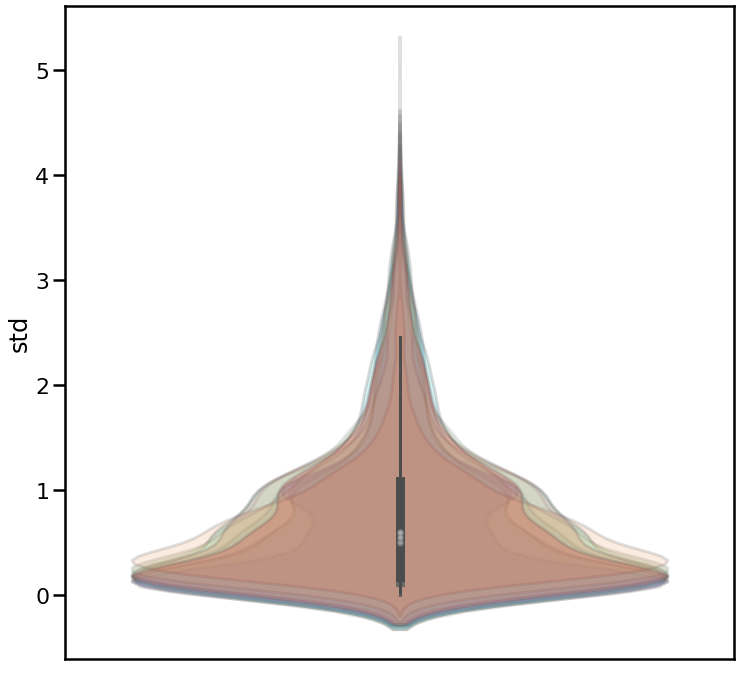
\includegraphics[width=0.5\linewidth]{../../result/mu_sigma_variance_plots/diann_log/diann_violinOverlap_qvalFiltered_pepFiltered_qbinned.png} & &%\includegraphics[width=0.3\linewidth]{} & 
%        D 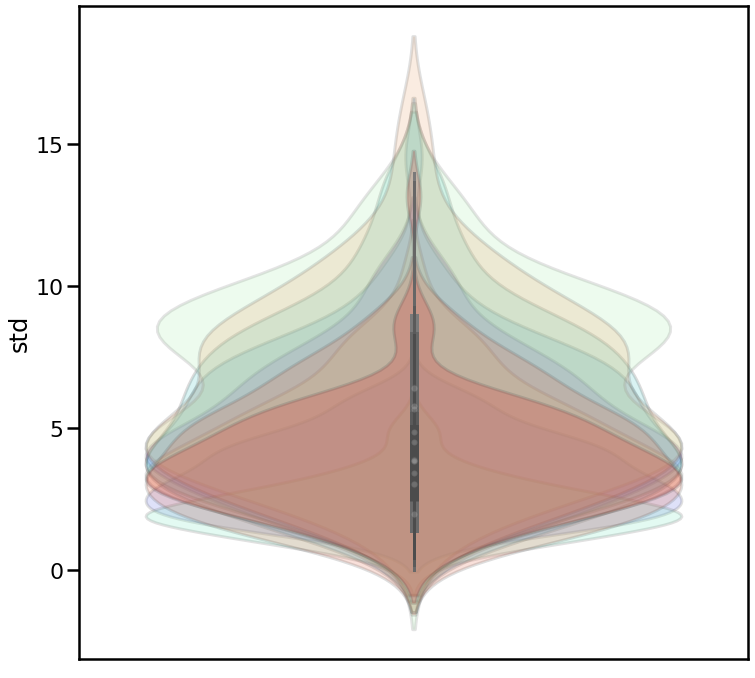
\includegraphics[width=0.5\linewidth]{../../result/mu_sigma_variance_plots/diann/diann_violinOverlap_nolog_qvalFiltered_pepFiltered_qbinned.png} & \\%\includegraphics[width=0.3\linewidth]{} \\ 
%    \end{tabular}
%  \caption{{\bf Overlapping violin plots of quantile binned peptide intensities.} We plotted overlapping violin plots of the quantile binned peptide intensities for (A-C) spectral library and (C-D) pseudo-spectra workflows. This despicts the same results as \ref{fig:mu_sigma_boxplot} and \ref{fig:mu_sigma_KDE}. \label{fig:mu_sigma_KDE}} 
%\end{figure}



% \begin{figure*}[t]
%      \centering
%      \begin{subfigure}{0.4\textwidth}
%        \includegraphics[width=\linewidth]{../FitData/ModelSelectionGraphs/Histogram_smad7_reproduced_BIC}
%        \caption{BIC}
%        \label{fig:model_selection:BIC}
%      \end{subfigure}
%      \begin{subfigure}{0.4\textwidth}
%        \includegraphics[width=\linewidth]{../FitData/ModelSelectionGraphs/Histogram_smad7_reproduced_RSS}
%        \caption{RSS}
%        \label{fig:model_selection:RSS}
%      \end{subfigure}
%      \caption{Distribution of Bayesian information criteria (BIC) and RSS values per model}
%      \label{fig:model_selection_criteria}
%    \end{figure*}

\end{document}
